\section{Direct connection to the selected CSA paper}
\label{sec:csa-bridge}
Our selected Part~1 paper proposes concurrent mode-wise subspaces for tensor-object reconstruction and recognition~\cite{csa}. Its projection/reconstruction equations, conditional eigenspace updates and Kronecker-constrained view of PCA provide a concrete mechanism to transfer. We add an exploratory experiment that directly calls the unchanged Part~1 \texttt{TensorCSA} implementation on LoRA functional responses. This extends the original project; it does not retrospectively turn the earlier merging algorithms into CSA.

\subsection{From image matrices to expert-response matrices}
For input $x$, we stack the four experts' base-subtracted, masked-mean final hidden responses into $X(x)\in\mathbb R^{4\times896}$. Expert identity and hidden coordinate are the two sample modes; the input-example axis is not a mode. No arbitrary reshaping of one vector into an image is used. With the fit mean $M$, CSA learns orthonormal $U\in\mathbb R^{4\times r_E}$ and $V\in\mathbb R^{896\times r_H}$:
\[
 C(x)=U^\top(X(x)-M)V,\qquad
 \widehat X(x)=UC(x)V^\top+M.
\]
The objective minimizes summed squared reconstruction error on the 512 fit examples. As in the selected paper's conditional updates, each mode is optimized with the other fixed. We reuse covariance initialization and an energy-based stopping rule from our Part~1 implementation, with at most 30 sweeps. These implementation conventions differ from the original paper's initialization/stopping details; convergence is not a global-optimum claim.

This is the same structured-representation mechanism as Part~1, now applied to a different tensor object. Hidden coordinates are shared by homologous backbones; successful separability is tested rather than assumed. We evaluate all seven predeclared rank pairs. The 512 fit, 512 selection and 1,024 internal-final examples per training seed match the existing role IDs. Bases are learned without fit labels; final responses are collected after router choices lock. All three teacher seeds are reused, so this is not three additional teacher replications or a pristine blind evaluation.

\subsection{Storage fairness and task usefulness}
For $E=4$, $H=896$ and $N=512$ cached objects, the full representation counts are
\[
 S_{\mathrm{CSA}}=EH+Er_E+Hr_H+Nr_Er_H,\qquad
 S_{\mathrm{PCA}}=EH+EHd+Nd.
\]
The mean is included in both. Arrays use float64, so scalar ratios compare like-for-like numerical storage; they are not ZIP compression ratios. We report both $d=r_Er_H$ and the largest integer PCA rank that fits within each CSA budget. Unused integer-budget remainder is retained. Same-latent PCA has a more general projection and is checked to have no higher fit reconstruction error. This reproduces Part~1's distinction between latent size and storage budget.

For downstream utility, each representation feeds a standardized logistic expert selector with known-task one-hot features. Fit targets are minimum-ground-truth-NLL experts; $C\in\{0.1,1,10\}$ uses selection native score only. Raw delta and base features receive the same router procedure, while task-ID remains a directly available reference. This is supervised, offline probing: constructing $X(x)$ requires all four expert forwards. Neither representation-cache savings nor router quality demonstrates faster deployment or compression of LoRA weights.

\begin{table}[htbp]\centering\small
\caption{Direct CSA transfer to expert-by-feature response matrices. Storage includes a fit mean, bases and 512 codes in float64. Reconstruction errors are relative squared errors on the previously explored internal final. Routing requires all four experts. Mean $\pm$ sample SD over three fixed teacher seeds.}
\begin{tabular}{lrrrr}\toprule
Representation & Latent & KiB & Rel. error & Native score \\ \midrule
csa2x8 & 16 & 148.1 & 0.4848 & 0.7080 $\pm$ 0.0250 \\
pca16 & 16 & 540.0 & 0.3843 & 0.7171 $\pm$ 0.0190 \\
pca3 & 3 & 124.0 & 0.5785 & 0.6966 $\pm$ 0.0646 \\
raw\_delta & -- & -- & -- & 0.6729 $\pm$ 0.0023 \\
base & -- & -- & -- & 0.6559 $\pm$ 0.0098 \\
task\_id & -- & -- & -- & 0.7695 $\pm$ 0.0114 \\
\bottomrule\end{tabular}\end{table}


\begin{figure}[htbp]\centering
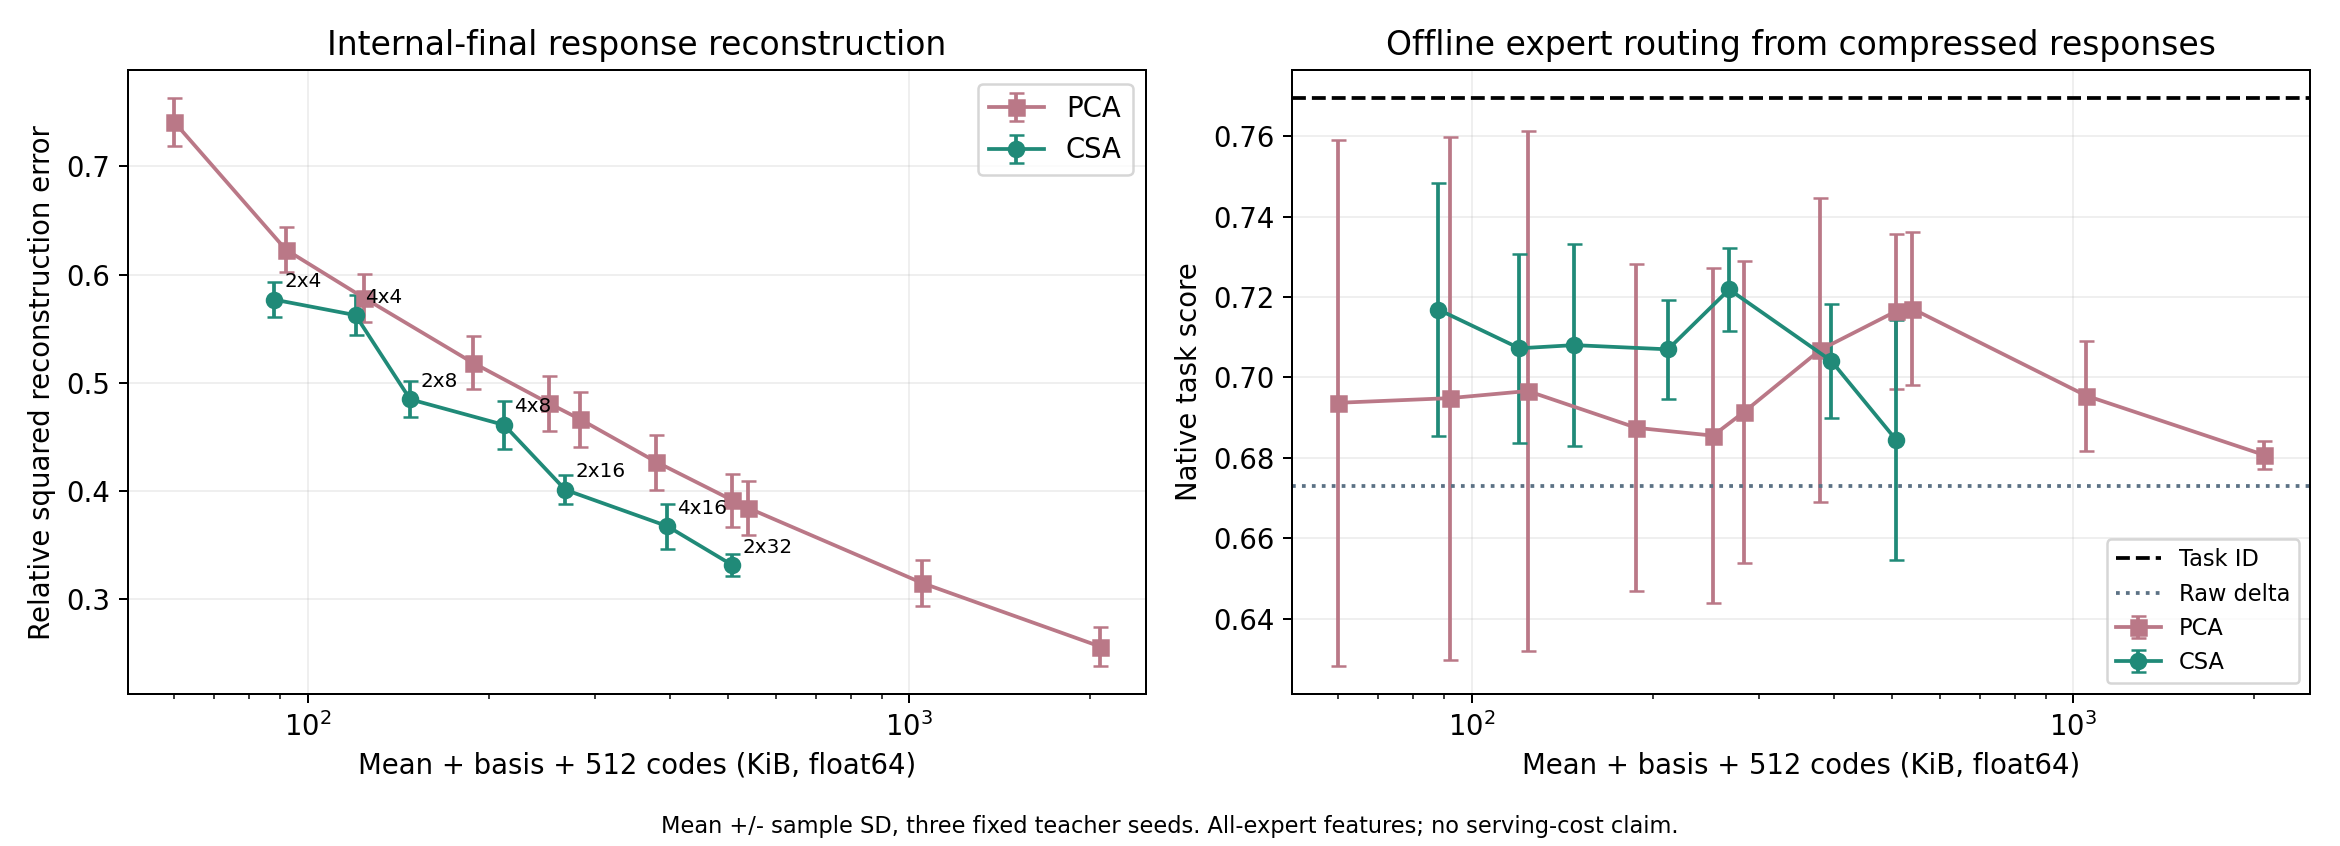
\includegraphics[width=\linewidth]{../artifacts/csa-bridge-2026-11-11/csa-storage-quality.png}
\caption{The direct CSA bridge: storage versus reconstruction and downstream information. Error bars are sample standard deviations over the same three teacher seeds. The storage scope excludes base/adapters, logits, router state and serialization.}
\end{figure}

For the illustrative $(r_E,r_H)=(2,8)$ setting, CSA stores 148.1 KiB, versus 540.0 KiB for equal-latent PCA, a 3.65-fold reduction in this representation scope. The largest budget-feasible PCA rank is 3. Internal-final relative squared errors are 0.4848 (CSA), 0.3843 (equal-latent PCA), and 0.5785 (budget PCA). Their native routing scores are 0.7080, 0.7171, and 0.6966, respectively; raw-delta routing is 0.6729 and task-ID is 0.7695. These comparisons separate representation compactness, reconstruction fidelity and task utility. The full predeclared grid is available in the evidence CSV; this illustration is not a final-selected best configuration.


The defensible link is now operational: Part~1 explains and tests structured tensor subspaces; Part~2 applies the same implementation to multi-adapter response objects and checks whether compact reconstruction preserves information useful for expert selection. The merge-weight study and this response-compression study answer complementary questions. We do not claim a new CSA algorithm, a CSA-based weight merger, or a free router.

